\documentclass[12pt]{report}
\usepackage{lmodern}
\usepackage[T1]{fontenc}
\usepackage{graphicx} % Allows you to insert figures
\usepackage{amsmath} % Allows you to do equations
\usepackage{fancyhdr} % Formats the header
\usepackage{geometry} % Formats the paper size, orientation, and margins
\usepackage[style=numeric,backend=biber,citestyle=numeric-comp,sorting=none,maxbibnames=99,giveninits=true,doi=true,isbn=false,url=false]{biblatex} 

\usepackage[colorlinks=true, linkcolor=black, citecolor=black, urlcolor=black]{hyperref}
\usepackage{booktabs}
\usepackage{appendix}
\usepackage[version=4]{mhchem}
\usepackage{listings} % For code
\usepackage{float}
\usepackage{subcaption}
\usepackage{wrapfig}
\usepackage[format=plain, font=it]{caption} % Italicizes figure captions
\usepackage[english]{babel}
\usepackage{csquotes}
\usepackage{titlesec}
\usepackage{comment}
\usepackage{indentfirst}

\AtEveryBibitem{
    \clearfield{urlyear}
    \clearfield{urlmonth}
    \clearfield{month}
    \clearlist{language}
} % Removes access date, months, and language from bibliography

\renewbibmacro{in:}{} % Removes the "In" before journal names

% Removed Harvard-specific settings and unnecessary macros:
% \citetrackerfalse % Not needed for numeric citations
% \DeclareNameAlias{sortname}{family-given} % Optional for Vancouver style, removed

% Vancouver-style superscript citations
\addbibresource{references.bib} % Specifies the bibliography file
\DeclareFieldFormat{labelnumber}{#1}
\renewcommand{\bibopenbracket}{}
\renewcommand{\bibclosebracket}{}
\renewcommand{\cite}{\supercite}
\renewcommand{\bibname}{References}
\DefineBibliographyStrings{english}{
  bibliography = {References}\textbf{}}

% Command to simplify images
\newcommand{\addimage}[4][0.8]{
    \begin{figure}[h]
        \centering
        \includegraphics[width=#1\linewidth]{Images/#2}
        \caption{#3}\label{fig:#4}
    \end{figure}
} % \simpleimage[ratio of linewidth (i.e. 0.5)]{image_name}{caption}{reference_name}

\newcommand{\addappendix}[2]{
    \chapter*{Appendix #1: #2}
    \addcontentsline{toc}{section}{Appendix #1: #2}
}

\newcommand{\setparindent}{
    \setlength{\parskip}{1em} % paragraphs separated by one line
    \setlength{\parindent}{2.5em} % no paragraph indents
}

% Title Formats
\titleformat{\chapter}[block]{\normalfont\large\bfseries\centering}{\thesection}{0.5em}{}
\titlespacing*{\chapter}{0pt}{0em}{0.5em}
\titleformat{\section}[block]{\normalfont\large\bfseries}{\thesection}{0.25em}{\vspace{-0.5em}}
\titleformat{\subsection}[block]{\normalfont\normalfont\bfseries}{\thesubsection}{0.25em}{\vspace{-0.25em}}
\titleformat{\subsubsection}[block]{\normalfont\normalfont\bfseries\itshape}{\thesubsubsection}{0.25em}{\vspace{-0.25em}}
% Remove chapter number from headings (due to report class)
\setcounter{secnumdepth}{3}
\setcounter{section}{0}
\renewcommand{\thesection}{\arabic{section}.}
\renewcommand{\thesubsection}{\arabic{section}.\arabic{subsection}.}
\renewcommand{\thesubsubsection}{\arabic{section}.\arabic{subsection}.\arabic{subsubsection}.}

% Paper Properties
\linespread{1.15} % about 1.5 spacing in Word
\setlength{\parskip}{1em} % paragraphs separated by one line
\setlength{\parindent}{2.5em} % no paragraph indents
\urlstyle{same} % makes a nicer URL and DOI font
\renewcommand{\headrulewidth}{0pt}
\geometry{letterpaper, portrait, margin=1in}
\setlength{\headheight}{14pt}

\raggedright % Removes justification completely
%\sloppy % Make the right edge sloppy, use \fussy to change back

\newcommand\titleofdoc{Non-intrusive Testing of Liquid Culture Medium using Online NIR Spectroscopy and Machine Learning for Qualitative Analysis} %%%%% Put your document title in this argument

\begin{document}
\begin{titlepage}
   \begin{center}
        \vspace*{2.5cm} % Adjust spacings to ensure the title page is generally filled with text

        \Large{\bfseries{\titleofdoc}} 

        \vspace{0.5cm}
            
        \vspace{3cm}
       
        \vspace{0.25cm}
        \large{Connor Reintjes, Paola Gonz\'alez P\'erez, Benjamin Samuel, Shiza Hassan}

        \vspace{0.25cm}
        \large{Supervisor: Dr. Amin Reza Rajabzadeh}
       
        \vspace{3 cm}
        \large{McMaster University, W. Booth School of Engineering Practice and Technology}
        
        \vspace{0.25 cm}
        \large{BIOTECH 4TR3 - Capstone}
       

       \vfill
    \end{center}
\end{titlepage}

\setcounter{page}{2}
\pagestyle{fancy}
\fancyhf{}
\rhead{\thepage}
\lhead{Reintjes, Gonz\'alez P\'erez, Samuel, Hassan}

\fancypagestyle{plain}{
    \fancyhf{} % Clear default header/footer
    \rhead{\thepage}
    \lhead{Reintjes, Gonz\'alez P\'erez, Samuel, Hassan}
    }

\chapter*{Abstract}
\setparindent

Insufficient quality assurance is a major expense associated with laboratories that can result in contamination, poor sample integrity, and lead to lost time due to repetitive sample testing. To ameliorate these issues, NIR spectroscopy has been combined with machine learning in this approach to qualitatively analyze the composition of liquid cultures in a non-intrusive and online manner. This will allow laboratories to save time by identifying contamination as soon as it happens and proceeding accordingly, as opposed to finding out after a full protocol has been performed. The method to achieve this involved creating a casing to house the NIR which would take spectra of the sample and pass it to a machine learning model that would then identify whether the sample is in a normal or contaminated state. In phase 1 of the experiment, the NIR housing was manufactured and initial testing was conducted for both contaminated and non-contaminated states, with the contaminant being Lactobacillus rhamnosus. The results achieved indicate that the NIR was able to differentiate between contaminated and non-contaminated samples. In phase 2, further data collection was conducted using a quartz cuvette and Teflon background to reduce noise and spectra interference. A data augmentation pipeline was constructed to overcome data size limitations. The processed data was then fed into a 1D-CNN model to obtain preliminary results on its performance. Implementation of one-class classification resulted in the overfitting of the model. The pipeline and 1D-CNN model will continue to be developed in order to improve their performance as more diverse data is collected.

\thispagestyle{empty}

\newpage
\tableofcontents
\thispagestyle{empty}
\newpage

\setparindent
\section{Introduction} % If you want numbered sections, remove the star after \section
Quality assurance issues are responsible for repeated testing, misdiagnosis, improper treatment and unpredictable costs.\cite{CostPoorQualityrandoxlaboratories} The contamination of samples is the most common problem experienced in microbial laboratories. The real-time monitoring of samples can represent a significant cost-saving solution to improve quality assurance practices in laboratory and industrial settings.\cite{ContaminationMicrobiologicalLaboratoryendeshawabatenh2018} To improve these issues, Near Infrared (NIR) spectroscopy has been combined with deep learning to provide real-time analysis of sample quality. This online analysis increases the testing and result obtention speed while remaining non-invasive to reduce further contamination of the samples.\cite{SpeechRecognitionUsingalsobhani2021} This technology also symbolizes a financial advantage by reducing the loss of biological samples using low computational requirements that can measure and classify the analyzed data as required. A deep learning model will be used to optimize this analysis as it offers advantages such as automatically integrating feature extraction, and incorporating hundreds of layers with many parameters compared to artificial neural networks.\cite{DeepLearningNearinfraredmishra2022}

The NIR spectral region has a range from 700 nm to 2500 nm. It is primarily characterized by absorption bands corresponding to the overtone and combination bands of \ce{C-H}, \ce{N-H}, \ce{O-H}, and \ce{S-H} stretching \autoref{fig:principle_bands}. Hence, the spectra of most compounds will show unique absorption peaks in the NIR spectral region. These peaks can be used for the quantitative and qualitative analysis of the compounds in gases, solids or liquids.

\begin{figure}[h]
    \centering
    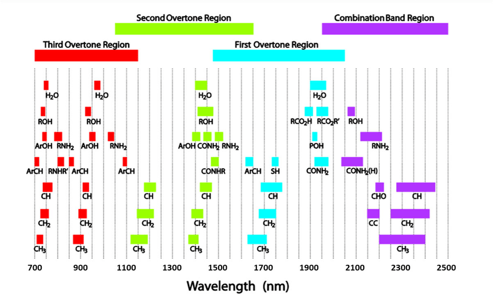
\includegraphics[width=0.75\linewidth]{Images/principle_bands.png}
    \caption{Principal analytical bands and relative peak locations for absorptions in the near-infrared region.\emph{NEEDS CITATION} Unique absorptions found in the majority of chemical and biological products can be utilized in both qualitative and quantitative examinations.}
    \label{fig:principle_bands}
\end{figure}

Ethanol and water have characteristic NIR spectrum patterns that allow for their identification and quantification as seen in \autoref{fig:anton_paar}. Ethanol has a unique narrow peak at $1200$ nm representing the second overtone of the \ce{C-H} stretching vibration.\cite{InfraredSpectroscopyNIR} Water, on the other hand, shows a flat behaviour at this wavelength due to the lack of \ce{C-H} bonds. 

The intensity of NIR absorption bands is $10-100$ times lower than that of the equivalent basic mid-IR absorption bands. This facilitates the direct analysis of strong absorbances and high light-scattering efficiency. Band overlap and penetration depth reduce in the near-infrared (NIR) spectral region, whereas the efficiency of light scattering and absorptivity improves with wavelength. As NIR spectroscopy depends on light absorption, spectral data can be acquired either in transmittance or reflectance mode. Diffuse reflectance $(\log \frac{1}{R} )$ measurements are favored for opaque or light-scattering matrices whereas translucent samples used transmittance $(\log \frac{1}{R})$.

\begin{wrapfigure}{r}{0.5\textwidth}
    \centering
    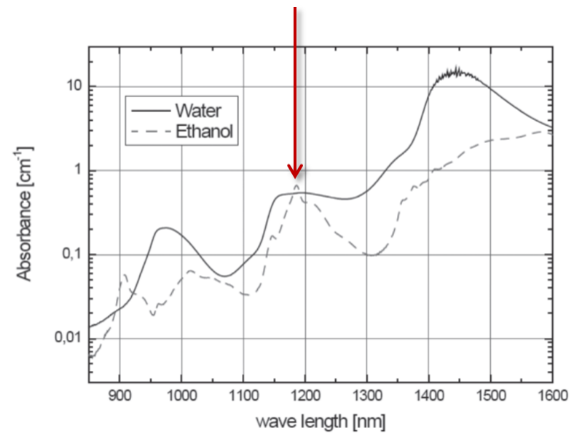
\includegraphics[width=0.48\textwidth]{Images/anton_paar.png}
    \caption{NIR spectrum of ethanol and water \cite{InfraredSpectroscopyNIR}}
    \label{fig:anton_paar}
\end{wrapfigure}

NIR spectroscopy's quickness, adaptability to a variety of materials, and capacity to examine liquid samples make it a promising tool for bio applications.\cite{NearInfraredSpectroscopyBioApplicationsbec2020} Recent advancements are making NIR spectroscopy more accessible with portable handheld instruments that allow for real-time, on-site examination. 
Cell culture media (CCM) plays a vital role, directly impacting process yield and product quality.\cite{CellCultureMediaryder2018} CCM's primary objective is to create and sustain an optimal physiological environment for large-scale cell culturing, ensuring cell health and expression of desired Critical Quality Attributes (CQAs). However, it's crucial to recognize that the chemical and physical properties of CCM are sensitive to microbial growth, chemical reactions, and environmental factors like temperature and light. Without sterilization, CCM can rapidly change due to microbial contamination, leading to increased turbidity and light scatter, consequently elevating baselines and noise in spectra, potentially compromising measurements. While chemometrics can mitigate some measurement errors, identifying errors induced by samples and measurements in CCM analysis can be challenging.

NIR spectra are known to be high-dimensional data due to the baseline drift and other noise signals present. This results in the need for preprocessing techniques for noise filtering and dimensionality reduction before analyzing the true compound signals.\cite{1DConvolutionalNeuralkrohling2023} Hence,  NIR spectra usually involve the use of chemometric algorithms like partial least squares regression (PLSR) and support vector regression (SVR) to clean the data from baseline drift as well as to understand the chemical changes in the samples.\cite{NIRSpectroscopyCombinedshang2023,LinearSupportVectornaguib2014} These algorithms require trained individuals to obtain the necessary parameters used to analyze the spectra.\cite{QuantitativeAnalysisYeastwang2017} Similarly, chemometric models are often limited by their inability to generalize for variance in spectra from different instruments, or changing storage and growing conditions. Deep Learning\cite{ReviewEvolutionChemometricswalsh2023} Machine Learning (ML) can be used to automate extracting the main compound features from high-dimensional spectral data and eliminate the need for feature-selection techniques. 
While different classes of ML algorithms have successfully achieved the classification of NIR spectra,\cite{1DConvolutionalNeuralkrohling2023} traditional ML methods such as partial least squares (PLS), K-nearest neighbor (KNN), and principal component analysis (PCA) require a higher level of expertise to design suitable features of the models architecture.\cite{zhangReviewMachineLearning2022} Deep learning, on the other hand, does not require a high level of expertise as it utilizes the raw features of data to analyze and classify it as needed. This is achieved through multiple hidden layers that are trained end to end. Some of these layers can be specialized convolution layers that allow for the learning and identification of local feature patterns. This aspect enables deep learning architectures to employ less preprocessing for high-dimensional data.\cite{FastDeepLearningyue2021} 

Convolutional neural networks (CNNs) are a class of deep neural networks commonly used for data analysis due to their successful results in image processing and classification,\cite{AnalysisConvolutionalNeuralsharma2018} speech recognition,\cite{SpeechRecognitionUsingalsobhani2021} and other computer vision tasks. CNNs are a feed-forward multi-layer architecture in which a kernel or filter takes specific features from local regions from the upper layer. This architecture allows for an autonomous extraction of important features from complex data for analysis and learning.\cite{NIRSpectroscopyCombinedshang2023} A common drawback of the use of CNNs for spectral analysis is the requirement of large data sets during the training process of the model.\cite{zhangNearInfraredSpectralCharacteristic2022} To avoid overfitting due to a limited number of data samples, one-dimensional CNN (1D-CNN) can be used. These models are similar to traditional CNNs except for the data size required and low computational requirements. 1D-CNNs have proven to have good information extraction and high classification accuracy with simple preprocessing techniques. It has been applied by Shang et al.\cite{NIRSpectroscopyCombinedshang2023} for the analysis and classification of NIR spectra from breast cancer tissue to aid in cancer diagnosis, demonstrating a $94.67\%$ classification accuracy. Chai et al.\cite{Improved1DConvolutionalchai2021} also developed an improved 1D-CNN structure to discriminate Anoectochilus roxburghii from its counterfeits using NIR spectra.

Previous studies performed on 1D-CNN for the analysis of NIR spectral data demonstrate the viability of its application for the online analysis of culture media. The present study aims to develop a method based on NIR spectra acquired on a portable device, as a non-destructive, online method to assess quality attributes of culture media. Due to the expected nature of the data collection, it was necessary to employ a time series analysis when designing the CNN structure. Within this experiment \emph{S. cerevisiae} was used as the model, testing it under two conditions, normal and contaminated with Lactic Acid Bacteria. \emph{Lactobacillus rhamnosus} was used as the contaminant of choice due to its improved growth in the presence of \emph{S. cerevisiae}. Also, using this species ensures the proper growth of \emph{S. cerevisiae} as it remains unaffected in its presence.\cite{YeastHumanCoevolutionnenciarini2024} The NIR spectra of ethanol were analyzed in each case and passed to the deep learning model which classified the “normal” baseline against a “non-normal” sample. 

\section{Methodology}
\subsection{NIR Housing Design}

Due to the design of the DLP NIRscan Nano (Texas Instruments) and the location of the sensor window on the unit, it required a housing to be designed. This housing was designed to both hold the NIR as well as the sample to ensure consistent scan conditions. The housing was created using a 3D printer (P1S, Bambu Labs) using Matte PLA filament (Bambu Labs) for the test models, and was reprinted in ABS filament (Bambu Labs) for the final housing.

The housing underwent multiple iterations with all design and modeling performed within AutoDesk Fusion360 parametric CAD software.\cite{Fusion360} The final iteration of the housing used can be seen below in \autoref{fig:nir_housing}. All of the components slide along a single dovetail mount along the bottom plate to allow for quick assembly while keeping all components secure. Due to slight problems with temperature regulation, a NF-A4x10 5V PWM fan from Noctua was added in addition to a fan speed controller (NA-FC1), to prevent the NIR from overheating during scans. A cuvette holder was also designed to allow for the quick change of samples, while also ensuring that the cuvette remained fixed in place for scans.

\begin{figure}[!h]
    \centering
    \begin{subfigure}[b]{0.4355\textwidth}
        \centering
        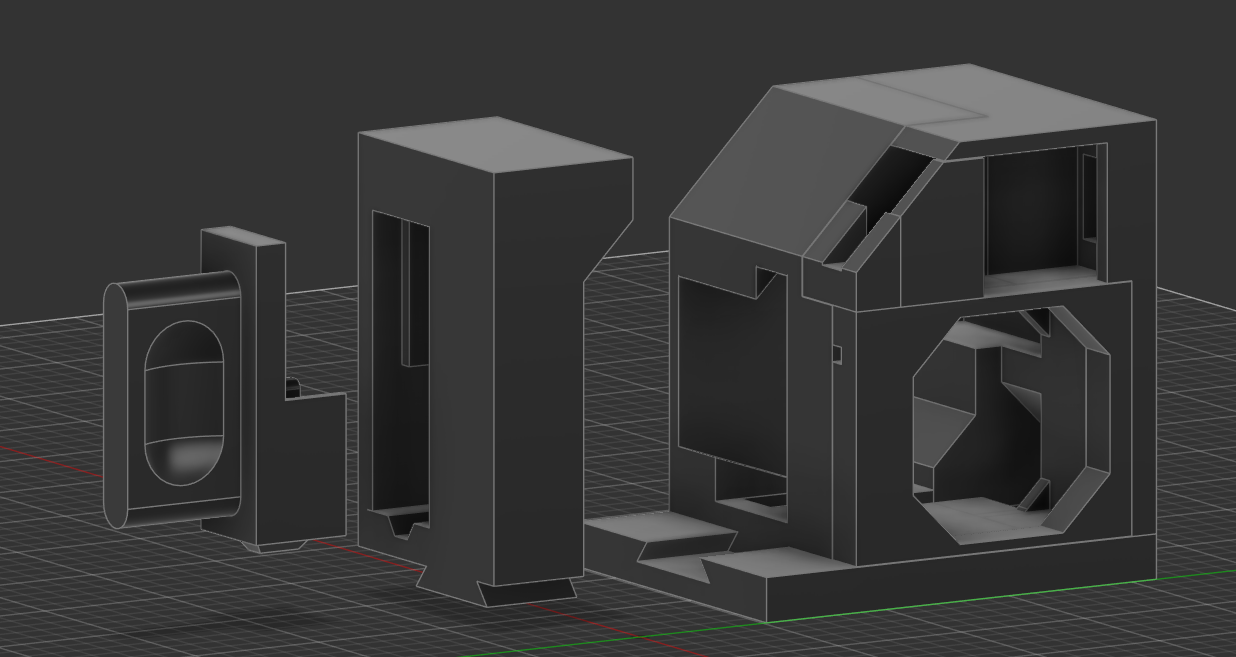
\includegraphics[width=\textwidth]{Images/nir_housing.png}  % Replace with your image file
        \caption{NIR Housing}
        \label{fig:nir_subfig1}
    \end{subfigure}
    \hfill
    \begin{subfigure}[b]{0.551\textwidth}
        \centering
        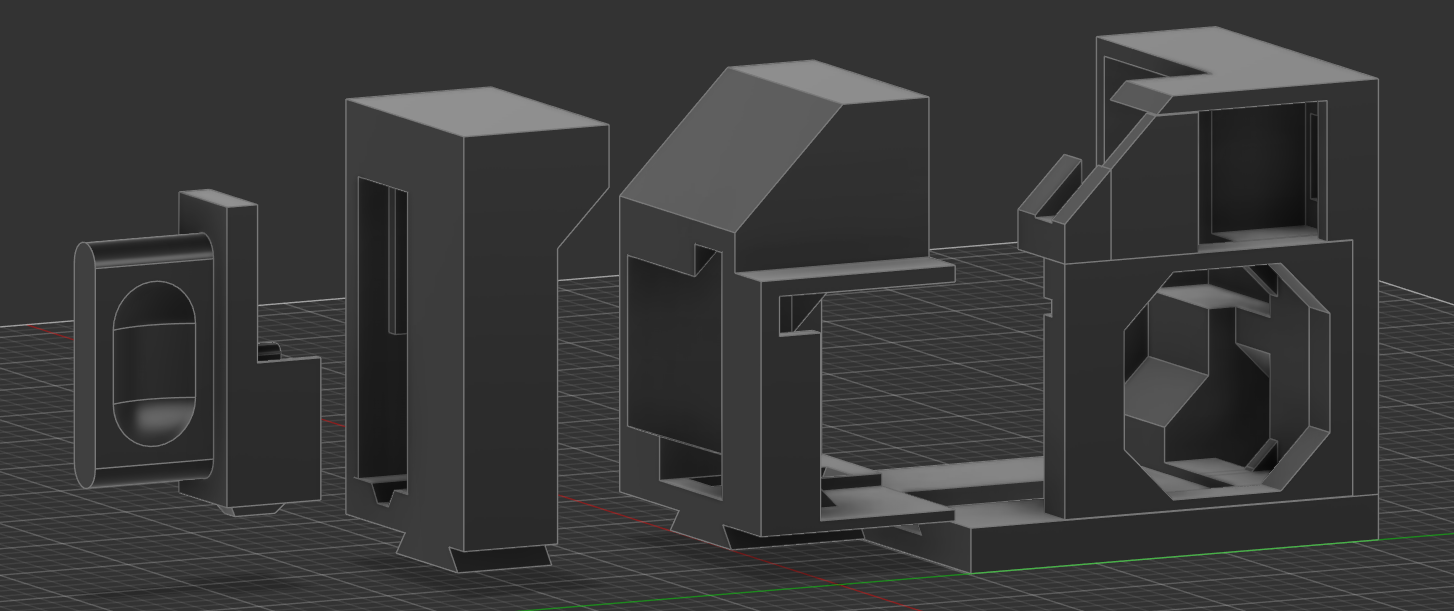
\includegraphics[width=\textwidth]{Images/nir_exploded.png}  % Replace with your image file
        \caption{NIR Housing Exploded}
        \label{fig:nir_subfig2}
    \end{subfigure}
    \caption{NIR Housing Design}
    \label{fig:nir_housing}
\end{figure}

The white PLA background was not as reflective as originally theorized, so the use of Teflon (PTFE) was considered. A high-reflectance PTFE sheet with 3M Adhesive backing was purchased from ThorLabs. This sheet has a reflectance $(> 90\%)$ in the UV spectrum,\cite{HighReflectancePTFESheetsthorlabs} and is one factor attributed to improving the signal-noise-ratio (SNR) within the scans.

\subsection{Ethanol Standard Curves}

To confirm the proof of concept of the project, ethanol standard curves were created and detected using the NIR to determine the differences in signals between different concentrations of ethanol. $6$ solutions of varying ethanol concentrations were tested in two stages, at higher concentrations and low concentrations. For the first standard curve, $300\text{mL}$ of distilled water was retained in a large beaker. Five, $100\text{mL}$ beakers were set up and labelled according to the scheme in \autoref{table:ethanol_water_high}. These volumes were added to each beaker and 3mL were subsequently taken out and placed into a plastic cuvette. The cuvette was cleaned with a kimwipe and then placed in the NIR to take a reading. The process was repeated for all beakers 3 times to generate 3 replicates for each sample. The concentrations used were far enough so it would make it easier to tell a difference between the absorbance readings taken from the NIR.

\begin{table}[!h]
    \centering
    \begin{tabular}{c c c}
    \toprule
    Sample & Ethanol Volume (mL) & Distilled Water Volume (mL) \\
    \midrule
    1 & 0   & 100 \\
    2 & 25  & 75  \\
    3 & 50  & 50  \\
    4 & 75  & 25  \\
    5 & 100 & 0   \\
    \bottomrule
    \end{tabular}
    \caption{Ethanol and Distilled Water Volumes for Initial Standards}
    \label{table:ethanol_water_high}
    \end{table}

For the second curve, smaller concentrations of ethanol were used to see if the NIR was able to detect small differences in concentrations of ethanol. The process was similar to the first standard curve. In this case, $600\text{mL}$ of distilled water was retrieved in a beaker and six, 100mL beakers were set up and labelled according to the scheme in \autoref{table:ethanol_water_low}. The remainder of the process was the same as before with the labelled volumes being added to each beaker and $3\text{mL}$ extracted to be placed in a plastic cuvette. The NIR spectra was taken and the process was repeated 3 times to generate 3 replicates. 

\begin{table}[!h]
    \centering
    \begin{tabular}{c c c}
    \toprule
    Sample & Ethanol Volume (mL) & Distilled Water Volume (mL) \\
    \midrule
    1 & 0   & 100 \\
    2 & 1  & 99  \\
    3 & 2  & 98  \\
    4 & 3  & 97  \\
    5 & 4 & 96   \\
    6 & 5 & 95   \\
    \bottomrule
    \end{tabular}
    \caption{Ethanol and Distilled Water Volumes for Low Concentration Standards}
    \label{table:ethanol_water_low}
    \end{table}

\subsection{Yeast Culture}

\subsection{\emph{Lactobacillus} Viability Test}

The Lactobacillus Rhamnosus viability test was conducted at the beginning of the term before running the experiments to ensure that the bacteria were alive when it came time to test the contaminated samples. This was performed by initially sterilizing the environment by lighting a Bunsen burner on an absorption mat. Then four MRS agar plates were inoculated with bacteria from the frozen samples from the previous term using an inoculating loop. Two samples each were taken from the hyperconcentrated and normal concentration samples, and one MRS plate was left untouched to serve as the control. The cells were evenly spread throughout the plate using a cell spreader to ensure even growth and the plates were then closed and wrapped with parafilm. They were then incubated at 37°C for 24 hours to allow for the bacteria to grow. 

\subsubsection{Lactobacillus Plating}

To prepare the contaminated cultures, a sterile environment was created by lighting a bunsen burner on an absorption mat, after which a hyperconcentrated sample of lactobacillus was retrieved from the freezer. An inoculating loop was used to pick up bacteria from the sample and placed on an agar plate, after which a cell spreader was used to spread the bacteria evenly across the plate. A second agar plate was also retrieved to serve as a control. Once the colonies were evenly spread the plate was closed, wrapped with parafilm and placed in an incubator for 24 hours at $37^{\circ}C$. After the incubation, the plate with lactobacillus was retrieved, and an inoculating loop was used to pick up colonies and place them in 20mL of YPD in an erlenmeyer flask. Afterwards, the flask was placed in a shaking incubator for 48 hours at $37^{\circ}C$. After 2 days the sample had reached confluency and 500uL were placed in test tubes after which the remaining was filled with YPD to reach a final volume of 3mL. The samples were then labeled and placed in the freezer at $-20^{\circ}C$ until they were needed for contaminated runs,   


\subsection{Spectral Measurement}

\begin{table}
    \centering
        \begin{tabular}{l c}
        \toprule
        Variable & Setpoint\\
        \midrule
        Start wavelength (nm): & $900$ \\
        End wavelength (nm): & $4.68$ \\
        Pattern Pixel Width (nm): & $1500$ \\
        Exposure (ms): & $1.27$ \\
        Digital Resolution: & $264$ \\
        Scan Repeats: & $9$ \\
        PGA Gain: & $64$ \\
        \bottomrule
        \end{tabular}
        \caption{Scan Setting for DLP NIRScan Nano}
        \label{tab:scaninfo}
\end{table}

\subsubsection{Spectral Processing}

Hadamard Transform is one of the available protocols built into the DLP NIRscan Nano. Unlike the column protocol which only reads one wavelength at a time, the Hadamard protocol takes a multiplex scan of multiple wavelengths simultaneously. An algorithm is then used to decode the individual wavelengths from the multiplex scan. The benefit of using Hadamard over Column is that Hadamard has a much better signal-noise ratio which will minimize the required preprocessing later.

\subsection{Data Pipeline}

\subsection{Convolutional Neural Network}

The classification of near-infrared (NIR) spectra to determine the contamination state of liquid media was performed with a one-dimensional convolutional neural network (1D-CNN). This neural network model uses the Keras library with Tensorflow as the backend. The use of Keras facilitates the modelling of the CNN due to its intuitive and user-friendly interface.\cite{kerasteam_keras} The Tensorflow backend allows for accelerated training when used with GPU.\cite{acecloudteam_2024_tensorflow} It also enables a detailed visualization through Tensorboard. Their combination results in a flexible model with easily customizable variables, like the layers and optimizers, along with shorter training times	

\subsubsection{Model Architecture}

The architecture of the model employs five different layers repeated at different points, as shown in figure x. The model consists of two Conv1D layers, with 64 and 32 filters respectively. These filters allow for the extraction of significant features in the input data.\cite{nisha_2020_applications} These features set the parameters that will be learned throughout training. To avoid overfitting and reduce the dimensionality of these parameters, MaxPooling1D layers and Dropout layers are implemented after the Conv1D layers.

The activation function, or function that transforms the input of a node into an output of that node, is a key component of a neural network. The model uses the Rectified Linear Unit (ReLU) function as the activation function, which only outputs non-negative outputs or zeros.\cite{brownlee_2019_a} This is commonly used in CNNs due to its ease of training and superior performance. A final dense layer is implemented with a sigmoidal activation function. This function outputs a probability score between 0 and 1 to determine the contamination state of the sample: 0 for non-contaminated and 1 for contaminated.\cite{saeed_2021_a} 

Figure x. 1D-CNN architecture diagram
\subsubsection{Optimizer and Loss Function}
Optimizers are functions responsible for adjusting the parameters as training progresses.\cite{eitcaacademy_2023_what} This is done to reduce the loss function, a mathematical quantification of the error margin between the prediction and the ground truth. The Adam algorithm was chosen as the optimizer. This follows a stochastic gradient descent based on adaptive estimation and regulated by the learning rate.\cite{kerasteam_keras} It allows for the model to reach an optimal point faster without taking large learning steps that could lead to skipping key information during training. The learning rate was set to 0.0005 to avoid reaching a convergence between the ground truth and prediction too early during training.

\begin{equation}
    L = -\frac{1}{N} \sum_{i=1}^{N} \left[ y_i \cdot \log(p(y_i)) + (1 - y_i) \cdot \log(1 - p(y_i)) \right]
    \label{eq:loss_function}
\end{equation}

The binary cross-entropy loss function was used in the model due to the binary classification nature of the project. The loss function is defined in \autoref{eq:loss_function}, where $y$ is the label $(1$ for contaminated and $0$ for non-contaminated$)$ and $p(y)$ is the predicted probability of the point being contaminated for all $N$ points. Binary cross-entropy quantifies the differences between the logarithmic probability distributions and penalizes inaccurate predictions which helps assess the model’s prediction confidence.

\section{Results}

\section{Discussion}

\section{Conclusion}

\begin{comment}
\begin{equation} % add * after equation for unnumbered equations
     \hat{H} \psi = i \hbar \frac{\partial \Psi}{\partial t}
\end{equation}

\begin{align} % good for multi-line equations. Alternatively use gather which centers equations
     \frac{D}{D_0} &= e^{-\frac{\mu}{\rho}\rho x} \\
    ln\left(\frac{D}{D_0}\right) &= -\frac{\mu}{\rho}\rho x \\
    x &= \frac{-ln\left(\frac{D}{D_0}\right)}{\frac{\mu}{\rho}\rho}
\end{align}
\end{comment}

\newpage
\printbibliography % If something looks strange in the bibliography, more often than not, you can modify the parameter in the .bib to fix the problem
\thispagestyle{empty}


\newpage
\appendix
\addappendix{A}{Problems}

As the experiment progressed, numerous changes were implemented in response to problems experienced in the laboratory. The initial plan involved using T25 flasks for fermentation and analysis. However, the spectra observed did not meet the theoretical composition analysis. Additionally, the volume of culture required was approximately 40 mL. This led to the experiment utilizing a cuvette for NIR spectroscopic analysis. 
The primary goal of this project was to carry out a Quantitative Composition Analysis. However, the lack of precise instruments, the spectra obtained did not have the sharpness and accuracy for quantitative analysis. This made it impossible to develop a prediction model and the project shifted focus to create a qualitative analysis.

Spectra for varying concentrations of glucose and ethanol were analysed. There were no observable differences in glucose production. As a result, the experiment, anaerobic fermentation was pursued and ethanol production was analysed to gain insight into the fermentation process in the cuvette. 
Plastic cuvettes were used for the qualitative analysis of the fermentation process as it was convenient and easy to establish a proof-of-concept. However, the spectra were not precise due to the reflection of light interfering with the results. In response, quartz cuvettes is proposed as a viable alternative for precise spectra. Important to note, that this has to be carried out yet. 
Throughout the experimental runs, there were technical issues encountered that directly impacted the frequency of results collected. The computer shut down after the first experiment. IT administration had to manually turn off that setting. For the following experiments, the computer restarts past 11:30 PM. As a result, the spectra would be taken only for 7-12 hours. For 2 runs, the NIR spectrometer was restarted the following day. Hence, there is unaccounted time in the fermentation process.

The final issue faced is the background is absorbing some of the light signals. Acrylonitrile Butadiene Styrene is the current background and it is used for 3D printing the NIR housing as it can withstand the heat generated from the NIR spectrometer. Two possible solutions can address this issue and will be implemented based on financial considerations. The first is to use a Teflon tape to prevent absorbance and maximize the reflectance. Alternatively, a transmittance module will be purchased to detect the signal and convert it to spectra

\addappendix{B}{Materials}

\begin{table}[H]
    \centering
    \begin{tabular}{l l l}
    \toprule
    Item & Supplier & Quantity\\
    \midrule
    DLP NIRscan™ Nano Evaluation Module & Texas Instruments & 1 \\
    Quartz Glass High Precision Cell & Hellma Analytics & 2 \\
    PTFE Diffuse Reflector Sheet with Adhesive Backing & ThorLabs & 1 \\
    ABS Black Filament & Bambu Labs & 1x 1kg \\
    \textit{S. Cerevisiae} & Sigma Aldrich & 100g \\
    \textit{Lactobacillus rhamnosus} & ATCC & 1 vial \\
    Peptone & Sigma Aldrich & 5g \\
    Yeast Extract & Sigma Aldrich & 5g \\
    Dextrose & Sigma Aldrich & 10g \\
    \bottomrule
    \end{tabular}
    \label{tab:matinfo}
    \end{table}

\end{document}
